
\chapter{Introduction}


% This has to be changed here rather than in the thesis.tex file since
% the 'chapter' command defines the new page where 'pagenumbering' will
% be effective
\pagenumbering{arabic}


\begin{chapterabstract}
This first part of this chapter starts with a brief general overview of the pnictides with particular focus on the `122' family and the \BaFePAs series. This includes a review of the pnictide Fermiology, how this relates to spin fluctuation mediated pairing and how the Fermiology of \BaFeP in particular is important to the understanding of these phenomena.

The second part of this chapter describes the cuprate phase diagram. In particular it outlines some important, apparently conflicting observations and some possible mechanisms to understand them. It also details previous work performed by the Bristol group on \acs{LSCO} and how performing high field measurements on \acs{BSCO} can provide further understanding of the mechanisms at work in the phase diagram.
\end{chapterabstract}


\subsection{The \BaFePAs series}

In order to explore the role of nesting in the high-$T_c$ superconductors, an investigation at Bristol was undertaken on the Fermiology of the \BaFePAs series by studying angle resolved \ac{dHvA} oscillations and in particular the end-member, \BaFeP.

The \BaFePAs series is one of many that stem from the parent compound \BaFeAs, although unlike the electron doped \BaCoFeAs and the hole doped \BaKFeAs series, the \BaFePAs progression is entirely isovalent meaning that the changes affected due to the P substitution are due to structure and chemical pressure rather than additional charge carriers. Nonetheless, superconductivity occurs with a very similar phase diagram as with the charge-doped examples in the same `$122$' family of iron-pnictide materials.\footnote{See for example figure~1 in ref.~\cite{Paglione2010}}. 

At $x=0$ the \BaFePAs series begins at \BaFeAs, a compound which becomes antiferromagnetic at around \unit{138}{\kelvin}, and moves with increasing $x$ towards \BaFeP which is metallic to low temperatures. Neither end members are superconducting, however as As is substituted for P, the low temperature antiferromagnetic state decays, giving way to superconductivity which kicks in at approximately $x=0.18$ and increases to the optimal substitution of $x=0.31$. Superconductivity then decreases until it gives way to a paramagnetic ground state at around $x=0.71$. Figure~\ref{Fig:Intro:PhaseDiagram} shows the phase diagram adapted from ref.~\cite{Nakai2010a} as determined by resistivity measurements. 
\begin{figure}[htbp]
    \begin{center}
        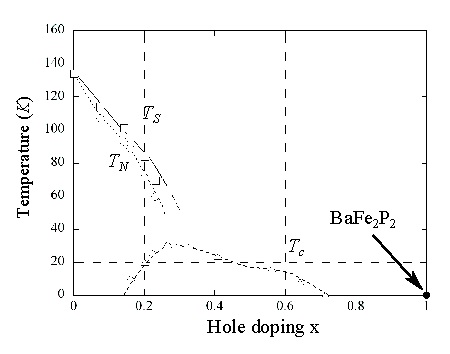
\includegraphics[scale=1.0]{Chapter-Introduction/Figures/PhaseDiagram/PhaseDiagram}
        \caption{Phase diagram adapted from ref \cite{Nakai2010a} measured by resistivity. $T_s$, $T_N$ and $T_c$ are the structural transition, the antiferromagnetic transition and the superconducting transition temperatures respectively.}
        \label{Fig:Intro:PhaseDiagram}
    \end{center}
\end{figure}
Also detailed in the phase diagram is the structural transition which occurs as the tetragonal $I4/mmm$ cell moves to an orthorhombic cell as it passes below the line marked $T_s$. This is a feature which is common to many of the `$122$' pnictide materials.

 The progression along the series is isovalent since P and As are in the same periodic group -- group $V$. The net effect of the substitution is to apply an increasing chemical pressure as $x$ moves towards $1$. Several reports show that applying high \emph{physical} pressure ($\sim$\unit{5}{\giga\pascal}) to \BaFeAs results in a similar phase diagram with an antiferromagnetic phase and superconductivity up to $\sim$\unit{30}{\kelvin}~\cite{Yamazaki2010,Colombier2009,Alireza2009} with Klintberg \etal~\cite{Klintberg2010} presenting a direct comparison between the two types of pressure. As pressure is applied, the unit cell $a$ axis shrinks slightly less than the $c$ axis ($\sim3\%$ cf. $\sim4.5\%$ respectively). Interestingly the $c$ axis shrinking largely occurs in the Fe-Pnictide plane leading to some theories of the superconductivity emerging from the tetrahedral bond angle between the Fe and the pnictogen.
\begin{figure}[htbp]
    \begin{center}
        \includegraphics[scale=1.0]{Chapter-Introduction/Figures/UnitCell/UnitCell}
        \caption{The tetragonal unit cell of the 122 \BaFePAs series clearly showing the tetragonally bonded Fe(As,P) layers.}
        \label{Fig:Intro:UnitCell}
    \end{center}
\end{figure}


The \BaFePAs series from a substitution of $x=0.41$--$1.0$ has been previously measured by members of the group at Bristol using dHvA oscillations\cite{Shishido2010}. As suggested in the Shishido reference, since dHvA has been observed across such a large range of substitutions, it implies that the material is not prone to disorder as is the case in many charge doped series \TODO{Need ref} making the series an excellent candidate for dHvA studies. This could be explained by the fact that the substitution is isovalent and that there is relatively little contribution at the Fermi surface from the pnictide sites\footnote{See for example, the orbital character for the iron sites from \ac{DFT} calculations presented later in this chapter} where the substitution takes place, meaning the Fermi surface should not be strongly disrupted when traversing the series. The Fermi surfaces from the Shishido paper have been characterised for x ranging from $0.41$ to $1$ for electron sheets only but have clearly shown that the DFT calculations consistently overestimate the size of the surfaces. They also show a linear progression of the electron orbit sizes which is proportional to $x$. Moreover, dHvA measurements on the material with $x=0.63$ have been performed where one of the hole surface extrema was observed\cite{Analytis2010c} however DFT calculations as well as comparisons with \SrFeP\cite{Analytis2009} give evidence for a second hole Fermi surface for materials towards the P end of the series, (towards the As end of the series, there appears this second hole and a \emph{third} hole surface similar but smaller to the other hole sheets). If the electron Fermi surfaces are oversized in the DFT calculations, then the hole Fermi surface volumes should also be oversized in order to remain compensated (electrically neutral). What is not clear though is whether the \emph{shapes} of the hole pockets are also altered in the compounds leading to \BaFeP. DFT calculations show the larger of the hole pockets in particular undergoing significant geometric changes, specifically in that it becomes much more three dimensional as P substitution becomes more complete. The Fermi surface of the opposite end-member, \BaFeAs, has been fully characterised by previous \ac{ARPES} measurements\cite{Kondo2010a} and dHvA\cite{Terashima2011, Analytis2010b}. Coupled with a full characterisation of the Fermiology of \BaFeP, this data can be used to interpolate Fermiology of the hole pockets between end members thus completing the partial determination of the Fermi surfaces of the intermediary compounds.

The \ac{ARPES} measurements of the Fermi surface of \BaFeAs below the N\'eel temperature concluded that despite some $k_z$ dispersion in the Fermi surfaces, there is adequate nesting to form the antiferromagnetic state. Ab-initio DFT calculations\cite{Shishido2010} of the paramagnetic state have shown the $k_z$ dispersion increasing with increasing P, with the outer hole pockets becoming more three-dimensional through the progression providing the partial nesting conditions necessary for pair forming \ac{SDW} fluctuations described in section\ref{Sec:1:Nesting}. One caveat is that these calculations do not take into account the structural changes below $T_s$, another caveat is that they do not consider Fermi surface reconstruction due to the observed commensurate antiferromagnetic order. To fully settle the issue of the nature of the nesting in the superconducting state, experimental determination of the Fermi surfaces of the series is necessary, a good guide to which can be obtained from study of the end-members.


This thesis presents data which details the full Fermi surface of \BaFeP including an elucidation of the shape of the 3D outer hole surface. Partial nesting is detailed between the outer hole surface and the inner electron surface with $q=(\pi, \pi, \pi/2)$ meaning the phenomenon persists through to the end member of the series. Also presented are effective mass measurements which show relatively small mass enhancements implying weak carrier correlations.


A \acf{SDW} is a magnetic ordered state of a solid analogous to, for example, ferromagnetism or antiferromagnetism. The ordering is a spatial modulation of the density of spin states with period $\vect{q}$ in momentum space\footnote{Care should be taken not to confuse \acp{SDW} with `spin waves' which are spin flip excitations in ordered magnetic states such as antiferromagnetism and ferromagnetism.}. Crucially the existence of the \ac{SDW} state depends on the nesting condition being present in the band structure of the material.

Nesting is the condition that occurs when similar sized and shaped cross sectional orbits of Fermi surface are mapped onto each other by a vector $\vect{q}$.



\section{Pairing mechaism}
\label{Sec:Intro:PairingMechanism}

Although there is good evidence that the anisotropic scattering term found in the \ac{ADMR} data could well be the scattering responsible for the pairing, the results do not make any claims as tot he nature of the scattering. The \ac{BCS} model explicitly states that the scattering is mediated by phonons in ceonventional superconductors however there are a few resons why this cannot be the sole scattering process in the \highTc materials.

\TODO{List some reasons why phonon is not enough}

Perhaps the most promising the candidate is the scattering off \ac{SDW} fluctuations which occur when a material is on the cusp of shifting into a a \ac{SDW} state. 



\section{The cuprate phase diagram}

Contrary to the recently discovered pnictide materials, the phase diagrams for the cuprates are very similar with principle differences being only in scale. However this universality comes with an greater abundance of features which are not present or at least have not yet been charactersised in the pnictides. Figure~\ref{Fig:Intro:PhaseDiagrams} shows the phase diagram for \TODO{Give a particular example that includes electron doping} in particular but the features are shared between the cuprates. Looking more closely at the hole doping side, which in general is where the superconductivity is more robust, we start in a Mott insulating antiferromagnetic \ac{SDW} state in the undoped parent compound, this gradually dissapates as doping is introduced along the temeprature scale, T$_N$



\section{Mott physics}

The Hubbard model takes the relatively simple and solvable tight-binding model and introduces an Anderson term which raises the energy for double occupancy by an amount $U$, known as the `Hubbard U'. This simple change deeply enriches the physics with one of the outcomes being the existance of the Mott insulating state which occurs when each lattice site is half filled with a single electron. The energy cost for an electron to hop to an adjacent site is so high that it locks the electrons in place, preventing effective conduction. Introducing holes (or electrons) allows once again hopping to take place and the eigenstates are no longer entireley localised.



\subsection{Properties of \acs{BSCO}}

The unit cell of the \highTc, doped cuprate \acf{BSCO} is illustrated in figure~\ref{Fig:Intro:BSCOUnitCell}. It is made up of layers as follows from the top; a BiO layer, then a SrO layer, then a CuO lattice common to all cuprates, then 2 BiO layers, a SrO layer, CuO, SrO, BiO. Variants of \acs{BSCO} include \ac{BSCO2212} and \ac{BSCO2213} which feature one and two extra CuO layers respectively. Most closely relatated in terms of structure is \acs{TL2201} which features Tl and Ba in place of Bi and Sr repsectivey.
\begin{figure}[htbp]
    \begin{center}
        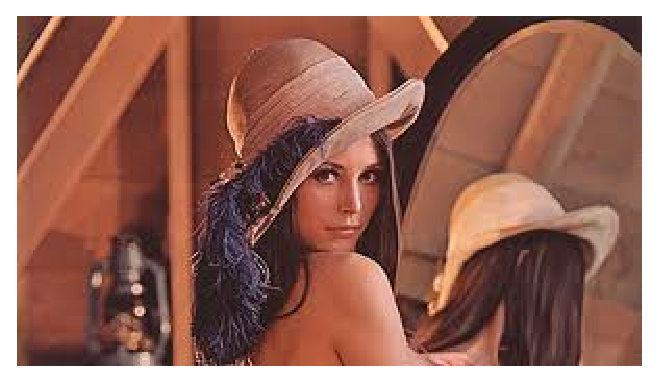
\includegraphics[scale=0.9]{Misc/TODO}
        \caption{Unit cell of \acs{BSCO}}
        \label{Fig:Intro:BSCOUnitCell}
    \end{center}
\end{figure}
Undoped \ac{BSCO} has an excess of holes and lies slightly to the undoped side of the phase diagram. By substituting in La for Sr, the amount of holes is reduced allowing access to a range of slightly overdoped to underdoped. However, since the substitution takes place adjacent to the CuO planes where all the interesting electronic behaviour happens, La doping introduces a lot of disorder into the system. Pb is also substituted for Bi which increases the number of holes alowing the more overdoped region to be accessed. Since Pb substitutes into the BiO layer which is far from the CuO plane, less disorder is introduced. Sometimes Pb is introduced alongside La even when a more underdoped state is desired since \TODO{Why not just dope lead? Was in the ARPES ref...}. Furthermore, annealing in oxygen decreases the number of carriers depending on how much additional oxygen is obsorbed allowing for even more fine grained tuning of the doping. By adjusting these parameters a very wide range of doping values can be accessed in \ac{BSCO} which makes it appealing for study.

The precise determination of doping from a chemical standpoint is tricky. For \ac{LSCO} --- assuming pure ionic donation --- substituting more Sr for La simply adds one more hole per extra Sr atom per unit cell. However for most other cuprates the heavy metal atom has a mixed valency meaning that the substitution relation is not so straightforward. Various techniques described in the methods section have been described to determine the doping level but as a rule some a priori knowledge of composition is required.

There is a crossover in overdoped curpates between a large hole-like Fermi surface to an electron-like Fermi surface that leads to a saddle point in the \ac{DOS} and consequently a van Hove singularity~\TODO{ref}. This occurs in \ac{LSCO} at around $p=0.18$ which is approximately critical doping and may lead one to believe that the critical behaviour is related to the proximity of the van Hove singularity. However the same crossover does not happen at the same doping in \ac{BSCO}, rather it appear to occur at $p \geq 0.2$, relatively far fromt he critical value of $p \approx 0.16$. For this reason \ac{BSCO} is an attractive material to study to determine more about the relationship (or lack thereof) between the critical behaviour and the van Hove singularity.




